\chapter{Анализ физических ограничений для решения задачи в ординарных каскадах}\label{ch:ch2}

Как уже было отмечено в главе 1, лишь некоторые из предложенных к настоящему моменту способов обогащения регенерированного урана потенциально способны решить такую задачу для произвольного исходного состава в условиях одновременного выполнения ограничений на концентрации сразу нескольких изотопов и при заданной пропорции между продуктом и исходной смесью. В первую очередь, это касается разбавляющих схем на основе ординарного каскада. 
Однако проведенный ранее теоретический анализ не позволяет однозначно утверждать при каких условиях может быть применена та или иная схема. В рамках настоящей главы описаны результаты серии вычислительных экспериментов и сопутствующего им теоретического анализа, направленных на то, чтобы выявить область возможного применения одиночных каскадных схем с разбавлением для получения обогащенного регенерированного урана в условиях многократного рецикла. 


\section{Постановка задачи и методическая часть}

Для изучения возможностей разбавляющих схем на основе ординарного каскада были рассмотрены случаи обогащения регенерированного урана с различных исходным содержанием чётных изотопов (см. \ref{is_compositions_2_5}). Выбранные составы соответствуют составам регенерированного урана, выделенных из ОЯТ реакторов ВВЭР-1000 и -1200 при различных внешних условиях \cite{palkinDesignanalyticalResearchRefinement2010,nevinicaToplivnyyCiklLegkovodnogo2019}. Отметим, что оба состава характеризуются довольно высоким содержанием $^{232}$U. Выбор подобных загрязненных четными изотопами составов регенерата иммитирует сложности, которые могут возникать при обогащении регенерированного урана в условиях многократного рецикла.  
При реализации вычислительных экспериментов общая постановка задачи соответствовала формулировке, приведенной в Главе 1. С учётом конкретных выбранных ограничений задачу можно сформулировать следующим образом.

Из заданной массы исходного регенерированного урана необходимо получить заданную массу товарного НОУ, отвечающего следующим требованиям:

\begin{enumerate}
  \item Требуемая концентрация в конечном продукте составляет 4.95\%, значение характерно для современных легководных реакторов \cite{solovevaCennostiOYaTKak2019}.
  \item Расход регенерированного урана на единицу конечного продукта в виде низкообогащенного урана: 0,93 кг на 1 кг НОУ \cite{smirnovApplyingEnrichmentCapacities2018}.
  \item Концентрация $^{235}$U в потоке отвала задана равной 0.1\% \cite{smirnovEvolutionIsotopicComposition2012};
  \item Соотношение $^{234}$U к $^{235}$U не должно превышать 0.02.
  \item Влияние изотопа $^{236}$U на нейтронно-физические характеристики топлива должно быть скомпенсировано дополнительным обогащение по $^{235}$U, для расчёта которого коэффициент компенсации реактивности принят равным 0.29 \cite{smirnovApplyingEnrichmentCapacities2018}.
  \item Концентрация $^{232}$U ограничена величиной $5\cdot10^{-7}$\%.
\end{enumerate}

В качестве схем обогащения регенерированного урана рассмотрены схемы, представленные на рисунке \ref{fig:diagram1}.
Каждая из них подразумевает использование ординарного каскада. Для моделирования процесса обогащения регенерированного урана в таком каскаде использовали модель R-каскада \cite{sulaberidzeTeoriyaKaskadovDlya2011}. При этом во всех случаях при расчёте параметров каскада задавали концентрации $^{235}$U в его внешних выходящих потоках. В этом случае под расчётом каскада параметров такого каскада подразумевали следующую задачу. 
Задано: состав обогащаемой смеси; параметры одиночного разделительного аппарата; величина одного из внешних потоков каскада, например, потока отбора или питания; концентрации $^{235}$U в потоках отбора и отвала каскада; в случае расчёта на основе модели R-каскада задают также пару компонентов, по относительным концентрациям которых выполняется условие несмешивания.
В процессе расчёта необходимо определить следующие параметры: число ступеней в каскаде и номер ступени подачи внешнего питания, концентрации всех компонентов (кроме $^{235}$U) в выходящих из каскада потоках, величины неизвестных внешних потоков каскада, распределения потока и концентраций компонентов по ступеням каскада и все остальные внутренние параметры. 
Такая постановка задачи требует численного решения системы нелинейных уравнений, возникающих для невязок концентраций $^{235}$U в выходящих потоках. Указанная система может быть записана в следующем виде: 

$\Delta_{P} = {(C_{235, P})}_{calc}-{(C_{235, P})}_{given}$
$\Delta_{W} = {(C_{235, W})}_{calc}-{(C_{235, W})}_{given}$

где $\Delta_{P}$, $\Delta_{W} - невязки по концентрациям $^{235}$U в потоках отбора и отвала каскада, соответственно. 
Для получения уравнений на невязки использованы соотношения (\ref{GrindEQ__1_72_}), (\ref{GrindEQ__1_73_}). Из решения подобной системы можно получить определить величины $(R_{n k}^{W}$ и $(R_{n k}^{P}$, после чего аналитически рассчитать остальные внешние параметры R-каскада по соотношениям (\ref{GrindEQ__1_70_})-(\ref{GrindEQ__1_77_}).   



\begin{table}[h]
  \centering
  \normalsize\begin{tabulary}{1.0\textwidth}{CCCCCCC}
  Цикл № & Массовое число & 232 & 233 & 234 & 235 & 236 \\
  2 & C, \% & 6.62e-7 & 1.19e-6 &    3.28e-2 & 1.43 & 0.9932 \\
   &  &  &  &  &  &  \\
  5 & C, \% &  1.03e-6 &   1.3e-6 &  3.91e-2 & 1.07 & 1.45 \\
   &  &  &  &  &  &  \\
  \end{tabulary}
  \caption{{Изотопные составы регенерата различных циклов.{\label{is_compositions_2_5}}}}
\end{table}


Ниже представлены результаты моделирования обогащения регенерата в каждой из трёх схем, представленных на рисунке 

.... 


\subsection{Схема с разбавлением предварительно обогащенного регенерата}

Рассмотрим каскадную схему, в которой регенерат сначала обогащают до уровня, превышающего требуемую концентрацию $^{235}$U, а затем разбавляют, например, природным ураном (рис. \ref{o1}). Такая схема позволяет обогатить регенерат до требуемого условием задачи содержания изотопа $^{235}$U в конечном продукте (НОУ), а также выполнить ограничения на $^{232}$U. При этом необходимо проверить соблюдение и остальных условий решаемой задачи обогащения регенерата.

\begin{figure}[ht]
  \centerfloat{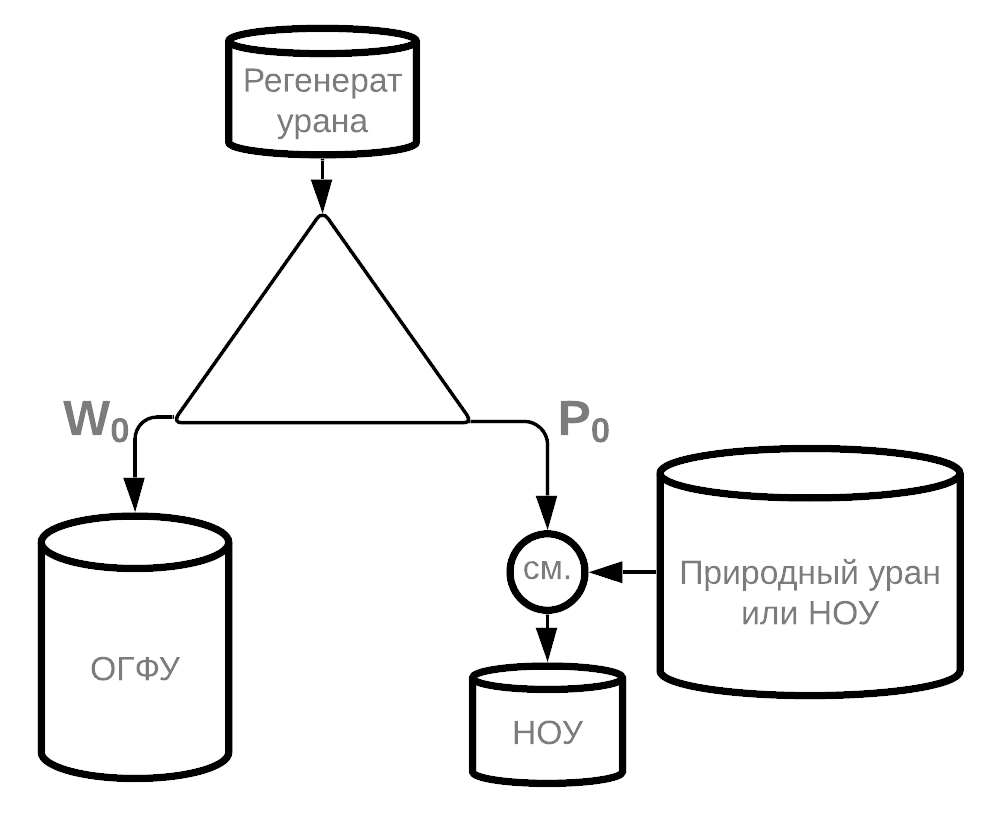
\includegraphics[scale=0.2]{cascades/ordinary/1}}
  \caption{Схема разбавления предварительно обогащенного регенерата природным ураном или низкообогащенным ураном. Обозначения: $P_0$ -- поток отбора легкой фракции каскада; $W_0$ -- поток отвального ОГФУ тяжелого конца каскада; $CM.$ -- узел смешения, на выходе из которого получается конечный продукт $НОУ$ -- низкообогащенный уран}\label{o1}
\end{figure}

Рассмотрим пример обогащения регенерированного урана, соответствующего второму рециклу. Для того, чтобы получить требуемый изотопный состав обогащенного урана, удовлетворяющий всем требованиям необходимо определить величину концентрации $^{235}$U в потоке $P_0$ и пропорцию смешивания. Указанные параметры определяли итерационно по следующей схеме. Сначала задавали начальное приближение для концентрации $^{235}$U в потоке $P_0$, после чего рассчитывали параметры каскада по описанной выше процедуре. Далее, зная состав смеси урана в потоке $P_0$ на основе простейшей пропорции определяли соотношение между потоками природного урана или обогащенного регенерата для получения финального продукта. При этом полученный в результате смешивания поток товарного НОУ должен отвечать ограничениям по концентрациям чётных изотопов. Это означает, что одновременно должны быть выполнены условия на концентрации изотопов $^{232,234,235,236}$U. Кроме того, для полного решения задачи должна быть обеспечена заданная пропорция между расходом регенерата и конечным продуктом. Однако управляющих параметров в такой схеме только два: концентрация $^{235}$U в потоке $P_0$ и пропорция смешивания обогащенного регенерата и природного урана. Очевидно, что в этом случае не для любых исходных данных возможно подобрать требуемые параметры каскадной схемы. 
Для иллюстрации приведенного выше утверждения

При этом Эта система задается невязками, связанными с достижением требуемой концентрации $^{235}$U в продукте, с учетом поправки на $^{236}$U: $C_{235 экв.}^{P}=C_{235 прир.}^{P}+\Delta C_{235}$, а также с выполнением ограничения на концентрацию $^{232}$U, задавая содержание этого изотопа в продукте равным предельно допустимому значению. С помощью такой системы уравнений, представленной на \ref{d1}-\ref{d2}, где ККР -- коэффициент компенсации реактивности, могут быть найдены числа ступеней в обогатительной и обеднительной частях каскада. Для решения указанной СНАУ можно подходит практически любой из известных численных методов решения СНАУ. 
При расчёте параметров ординарного каскада во всех случаях предполагали, что в каскаде было реализовано несмешивание по относительной концентрации компонентов $^{235}UF_6$ и $^{236}UF_6$. Такое условие было выбрано на основе серии предварительных расчётов. Величину коэффициента разделения для компонентов  $^{235}UF_6$ к $^{238}UF_6$ приняли равной 1.2  \cite{smirnovEvolutionIsotopicComposition2012}. 

\begin{equation} \label{d1} 
  \delta_1=\left[C_{235}^P-\left(C_n^P+KKP\times C_{236}^P\right)\right]
\end{equation} 

\begin{equation} \label{d2} 
    \delta_2=\left[C_{232}^P-5\times10^{-7}\right]\times10^5.             
\end{equation}


поскольку уравнений используемых для описания такой схемы меньше, чем условий, представляющей из себя систему нелинейных уравнений с невязками $\delta_1$, $\delta_2$ \ref{d1}-\ref{d2}, где ККР -- коэффициент компенсации реактивности, только два:

\begin{enumerate}
  \item выходная концентрация $^{235}$U обогащаемого регенерата;
  \item соотношение смешиваемых потоков $P_0$ и природного урана.
\end{enumerate}

Эти параметры в ходе вычислений будут варьироваться в доступных для них диапазонах для возможности найти решение или подобрать наилучшее решение. Величина концентрации U-235 в потоке отвала каскада фиксируется на уровне 0.1\%. 

При этом важно отметить, что хоть выходная концентрация $^{235}$U и является управляющим параметром, ее изменение неминуемо влечет за собой изменение и концентраций $^{236}$U и $^{232}$U, тем самым внося дополнительную неопределенность в решение задачи.

Это значит, что нахождение строго удовлетворяющего всем условиям решения не гарантировано и зависит от исходного состава регенерированного урана, а также требования к концентрации продуктового НОУ.

Результаты вычислительных экспериментов с помощью модели R-каскада, проделанных для обогащения состава второго рецикла, показали, что для данного состава не удалось найти решение задачи, которое бы одновременно отвечало требованиям на концентрации изотопов $^{232,234,236}$U в конечном НОУ-продукте. Невозможность нахождения подобного решения иллюстрируют кривые представленные на рис. \ref{delta1}-\ref{delta4}.

Они отражают зависимости величин $\delta_1$ и $\delta_2$ \ref{d1}-\ref{d2} от соотношения смешиваемых потоков, взятых для различных значений концентрации $^{235}$U (рис. \ref{delta1}--\ref{delta4}) в обогащенном регенерате.



По своему физическому смыслу величина $\delta_1$ представляет собой абсолютное отклонение концентрации изотопа $^{235}$U (выраженное в долях) в окончательном продукте (после смешивания) от требуемой величины, с учетом компенсации $^{236}$U, а величина $\delta_2$ представляет собой разность фактической концентрации $^{232}$U в окончательном продукте и требуемой величины в соответствии с принятым ограничением. Чтобы сопоставить указанные величины на одном рисунке, $\delta_2$ была взята с поправкой (умножена на специально подобранный числовой коэффициент). То есть, величины $\delta_1$ и $\delta_2$ соответствуют невязкам в решении системы нелинейных уравнений, которые, в случае нахождения решения системы будут равняться нулю (величине, не превышающей максимально допустимую погрешность вычислений, которая в численном методе решения задается с помощью специальной системной переменной).

\begin{figure}[ht]
  \begin{minipage}{.5\textwidth}
    \centering
    % include first image
    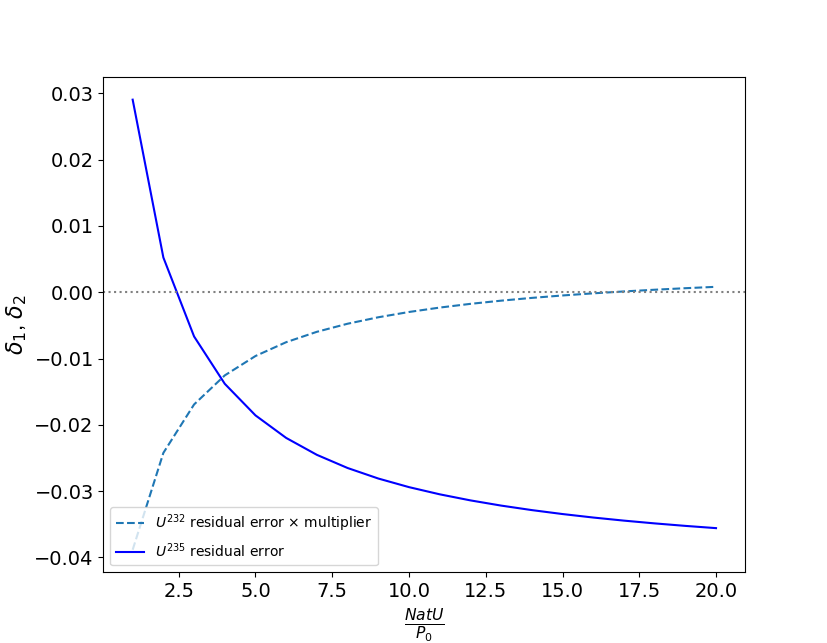
\includegraphics[width=.8\linewidth]{images/plots/15}  
    \caption{Концентрация $^{235}$U в предварительно обогащенном регенерата равна 15\%}
    \label{delta1}
  \end{minipage}
  \begin{minipage}{.5\textwidth}
    \centering
    % include second image
    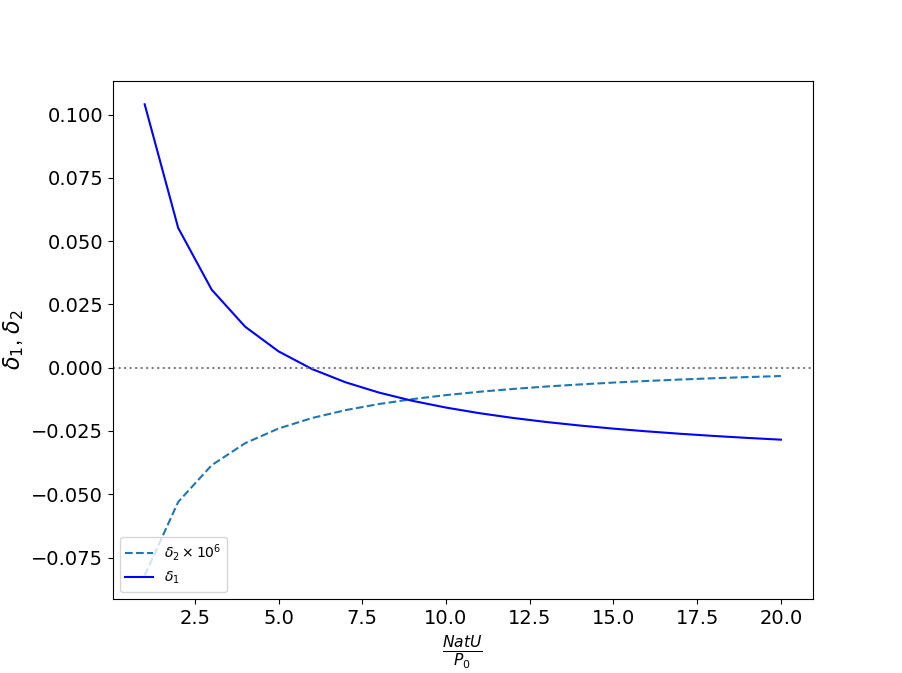
\includegraphics[width=.8\linewidth]{images/plots/30}  
    \caption{Концентрация $^{235}$U в предварительно обогащенном регенерата равна 30\%}
    \label{delta2}
  \end{minipage}
  \begin{minipage}{.5\textwidth}
    \centering
    % include second image
    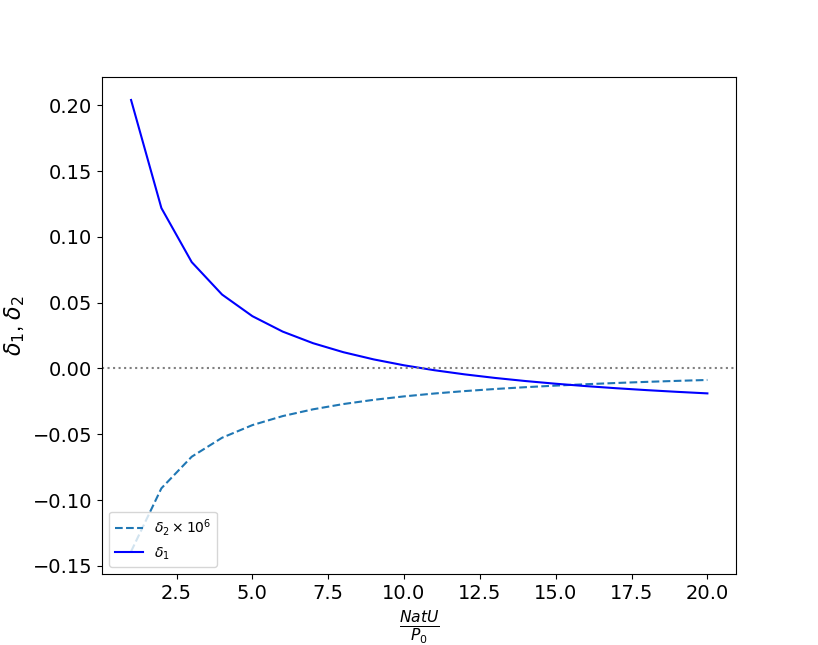
\includegraphics[width=.8\linewidth]{images/plots/50}  
    \caption{Концентрация $^{235}$U в предварительно обогащенном регенерата равна 50\%}
    \label{delta3}
  \end{minipage}
  \begin{minipage}{.5\textwidth}
    \centering
    % include second image
    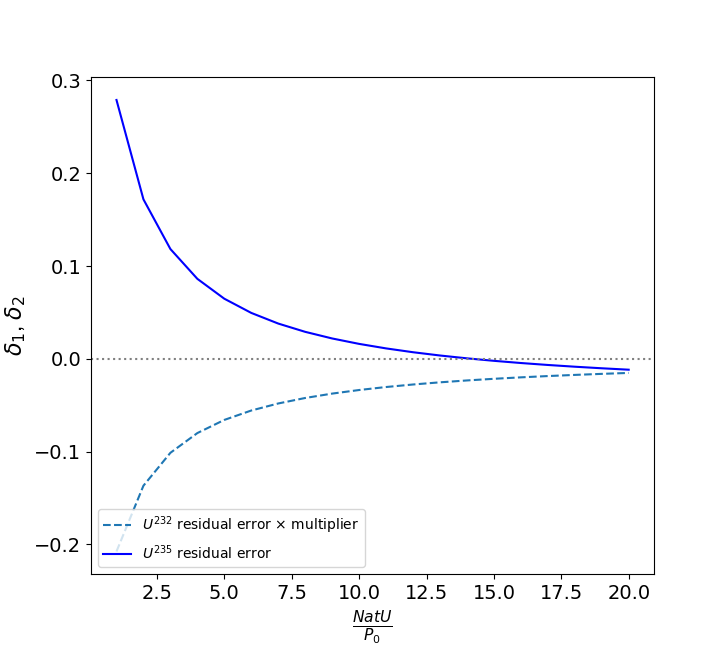
\includegraphics[width=.8\linewidth]{images/plots/65}  
    \caption{Концентрация $^{235}$U в предварительно обогащенном регенерата равна 65\%}
    \label{delta4}
  \end{minipage}
  % \caption{Невязки для $^{235}$U и $^{232}$U. Обозначения: $\frac{NatU}{P_{0}}$ -- отношение доли природного урана к потоку обогащенного регенерата.}
  % \label{fig:deltas_ordinar}
 \end{figure}

Для успешного решения СНАУ, определяемой системой двух нелинейных уравнений с невязками $\delta_1$ и $\delta_2$ \ref{d1}-\ref{d2}, обе эти величины должны равняться нулю для одного и того же значения аргумента функции (ось  Х), чего не удается достичь для рассмотренного состава, что и иллюстрируют рисунки \ref{delta1}-\ref{delta4}.

Таким образом, полученные результаты показывают невозможность применения каскадной схемы с разбавлением обогащенного регенерата природным (рис. \ref{o1}), когда будут одновременно выполнены условия на $^{235}$U и $^{232}$U, для решения задачи для данного изотопного состава. Иными словами, из-за принципиальных ограничений схем, основанных на ординарном каскада, с их помощью невозможно осуществить возврат всего регенерата в ядерный топливный цикл в условиях многократного рецикла.

\subsection{Схема с разбавлением предварительно обогащенного регенерата низкообогащенным ураном}

Если в схеме, рассмотренной выше (рис. \ref{o1}), заменить разбавитель предварительно обогащенного регенерата (рис. \ref{o1}) с природного урана на низкообогащенный уран, не содержащий четных изотопов (например, изготовленный из природного урана), для данного состава найдется решение, когда одновременно выполнены условия равенства нулю обеих невязок ($\delta_1$ и $\delta_2$). Нахождение решения для такой схемы обусловлено появлением дополнительного управляющего параметра -- концентрации $^{235}$U в потоке $НОУ$-разбавителя.

Чтобы исследовать область допустимых значений параметров схемы, а также определить при каких параметрах схема наиболее эффективна, исследованы диапазоны изменения следующих параметров схемы: $^{235}$U в концах каскада: $P_0$ и $W_0$ (рис. \ref{o1}). Это поможет проиллюстрировать как меняются доли природного урана и регенерата в конечном продукте и как меняются затраты работы разделения, за счет изменения длины каскада. Это позволит исследовать возможность достижения заданной пропорции возврата регенерата. 

\begin{figure}[ht]
  \centerfloat{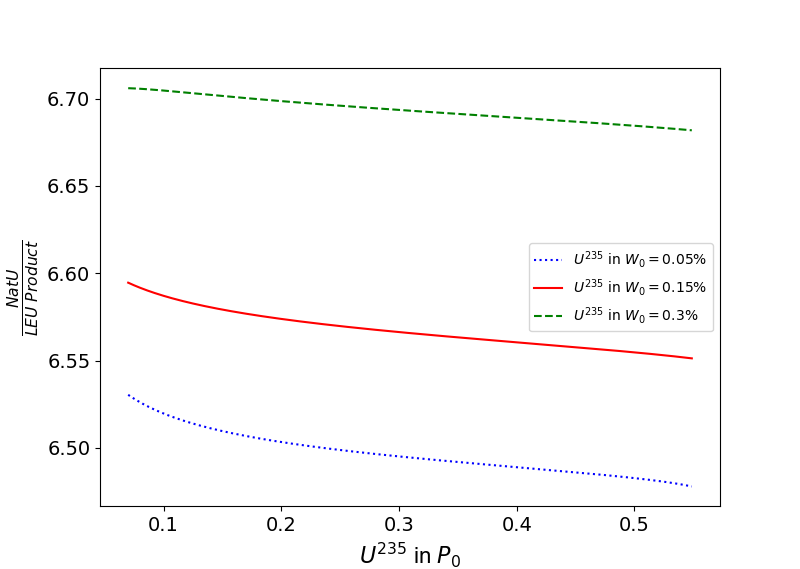
\includegraphics[scale=0.5]{images/plots/sc2_2}}
  \caption{Расход природного урана на единицу НОУ-продукта  для различных концентраций $^{235}$U в потоках продукта и отвала каскада, обогащающего регенерат}\label{fig:sc2_2}
\end{figure}

Рис. \ref{fig:sc2_2} иллюстрирует зависимость расхода природного урана (NatU) на единицу НОУ-продукта (LEU Product) от концентрации $^{235}$U в обогащенном регенерате ($P_0$ на рис. \ref{o1}) для разных значений концентрации $^{235}$U в отвале каскада, получаемом из регенерата. Значения уровня расхода природного урана на единицу НОУ-продукта на уровне $\approx$6,5-6,7 для всего исследуемого диапазона параметров, меньше, чем расход природного урана в схеме ординарного каскада ($\approx$7,93 на ед.продукта, смотри Приложение), когда он используется без добавки из регенерата для производства свежего НОУ топлива, аналогичного по исходным требованиям к продукту. Для значений концентрации $^{235}$U в $W_0$ на уровнях 0,05\% и 0,15\%, значения расхода природного урана в схеме ординарного каскада для обогащения природного урана, будут составлять $\approx$7,41 и $\approx$8,55, соответственно. Таким образом, при заданном интервале параметров, использование схемы с разбавлением обогащенного регенерата позволяет обеспечить экономию природного урана на уровне 15--28\%, что говорит о целесообразности использования регенерата в производстве НОУ.

Заметим, что по $^{235}$U регенерат обогащается до значений (рис.  \ref{fig:sc2_2}), превышающих пороговое значение для НОУ в 20\%, что может быть неприемлемым в виду требований соблюдения условий нераспространения ядерных материалов \cite{brownOriginsSignificanceLimit2016}. Именно эти значения соответствуют наилучшим показателям экономии природного урана, хотя переход 20\%-й границы для $^{235}$U, дает прирост экономии природного урана менее 1\%. Более существенное улучшение экономии (>3\%), как видно на графике \ref{fig:sc2_2}, происходит с ростом уровня извлечения $^{235}$U из регенерата при понижении концентрации $^{235}$U в обедняемом потоке регенерата $W_0$. 
% Эффект экономии природного урана от понижения $^{235}$U в $W_0$, а также от повышения $^{235}$U в $P_0$, обсуловлен возможностью использовать НОУ-разбавитель с более низким уровнем $^{235}$U, что проиллюстрировано на рис.\ref{fig:sc2_LEU_D}.

Уменьшение концентрации $^{235}$U в обедняемом потоке регенерата $W_0$ связано с еще одним преимуществом: более высокий уровень обеднения исходной смеси ($^{235}$U в $W_0$ при концентрации 0,05\%), дает существенный вклад в экономию работы разделения, что показано на рис.\ref{Figure_13}, за счет более эффективного извлечения $^{235}$U из регенерата. Область отрицательных значений потерь работы разделения (SW loss) на рис. \ref{Figure_13} соответствует ее экономии. Слияние кривых, соответствующих различным концентрациям $^{235}$U в обогащенном регенерате, обусловлено эквивалентностью масс $^{235}$U в каждом из этих потоков, что отражает постоянство вклада обогащенного регенерата в формирование конечного продукта, и соответствует постоянному уровню извлечения $^{235}$U.

% \begin{figure}[ht]
%   \centerfloat{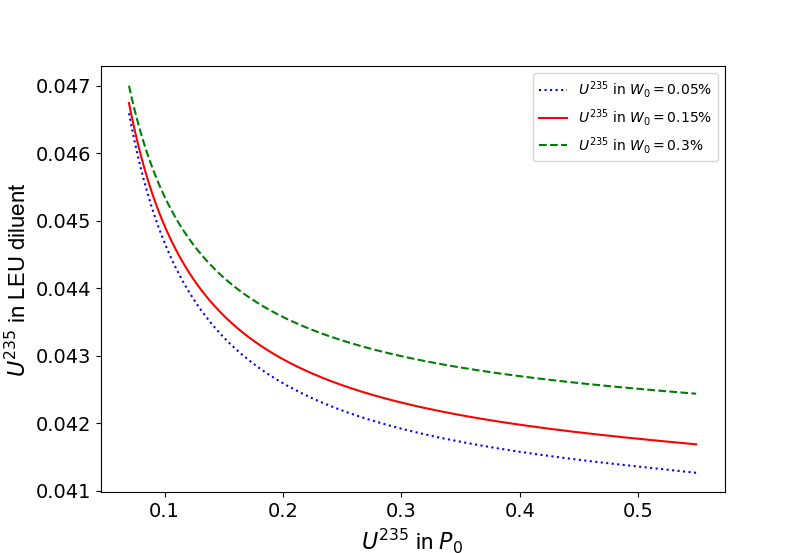
\includegraphics[scale=0.5]{images/plots/sc2_LEU_D}}
%   \caption{Концентрация $^{235}$U в разбавителе, необходимая для получения свежего НОУ для различных концентраций $^{235}$U в потоках продукта и отвала каскада, обогащающего регенерат}\label{fig:sc2_LEU_D}
% \end{figure}


\begin{figure}[ht]
  \centerfloat{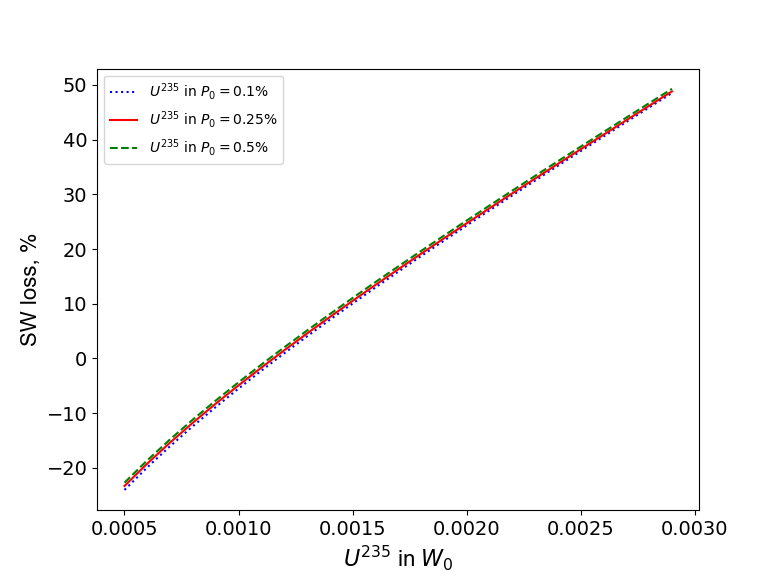
\includegraphics[scale=0.5]{images/plots/Figure_13}}
  \caption{Потери работы разделения по отношению к ординарному каскаду для обогащения природного урана для различных концентраций $^{235}$U в потоках продукта и отвала каскада, обогащающего регенерат}\label{Figure_13}
\end{figure}

Анализ графика \ref{Figure_10} зависимости расхода регенерата на единицу НОУ-продукта ($\frac{NatU}{P_{0}}$) от концентрации $^{235}$U в $W_0$, показывает невозможность выполнить условия возврата заданной доли регенерата на единицу продукта при любых параметрах каскадной схемы ($^{235}$U в $W_0$ и в $P_0$). Причем пропорция используемого регенерата к НОУ-продукту меняется лишь незначительно концентрацией $^{235}$U в $W_0$, а удлинение обогащающей части каскада (рост $^{235}$U в $P_0$) не приводит росту вовлечения регенерата.

\begin{figure}[ht]
  \centerfloat{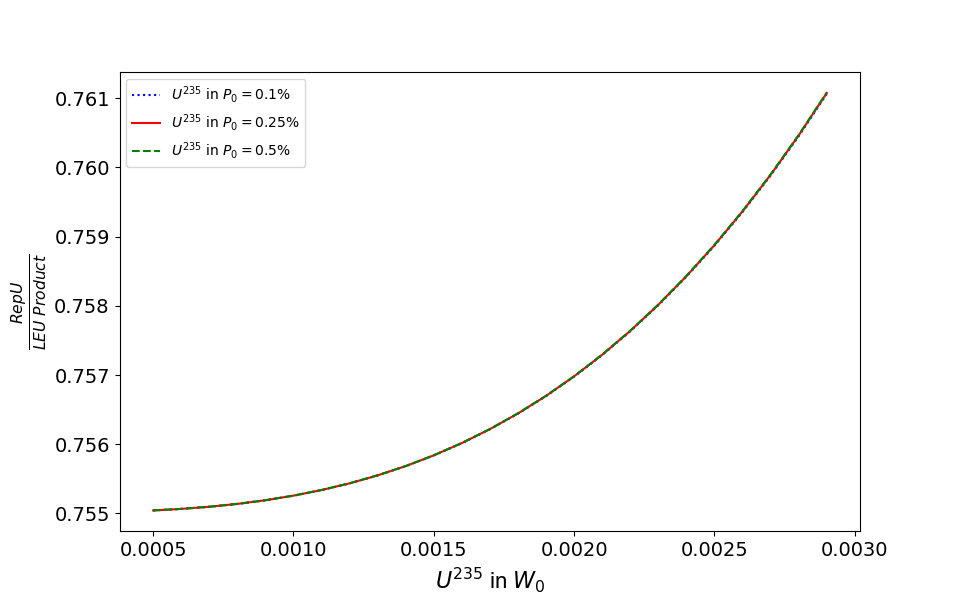
\includegraphics[scale=0.5]{images/plots/Figure_10}}
  \caption{Расход регенерата на единицу конечного НОУ-продукта для различных концентраций $^{235}$U в потоках продукта и отвала каскада, обогащающего регенерат}\label{Figure_10}
\end{figure}

% Проиллюстрировать затраты на работу разделения от составных  частей каскадной схемы, можно с помощью рис.\ref{myplot}, который показывает, что доля центрифуг для приготовления разбавителя из природного урана выше, чем доля центрифуг, задействованных для предварительного обогащения регенерата, и эта пропорция уменьшается с понижением содержания $^{235}$U в $W_0$.

% \begin{figure}[ht]
%   \centerfloat{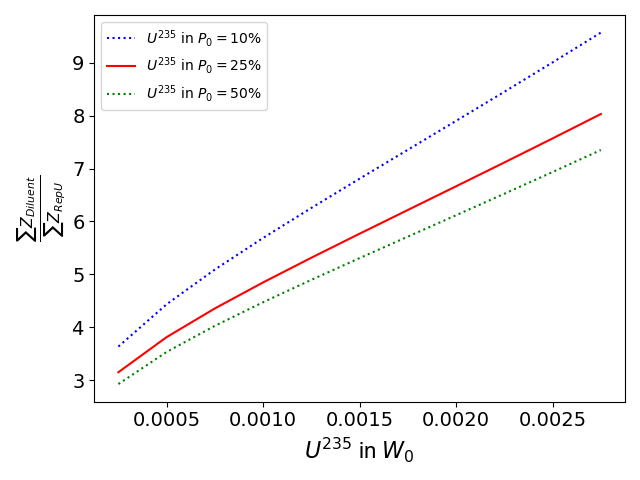
\includegraphics[scale=0.5]{images/plots/myplot}}
%   \caption{Отношение количества центрифуг в каскаде, производящем разбавитель из природного урана, к количеству центрифуг, задействованных для предварительного обогащения регенерата, для различных концентраций $^{235}$U в потоках продукта и отвала каскада, обогащающего регенерат}\label{myplot}
% \end{figure}

На основе анализа рис.\ref{fig:sc2_2}-\ref{Figure_10}, можно заключить, что схема с разбавлением обогащенного регенерата смесью, не содержащей минорных изотопов, непригодна для решения задачи обогащения в условиях многократного рецикла, так как с помощью нее нет возможности использовать весь регенерированный уран на производство НОУ-продукта, как показано на рис. \ref{Figure_13}.

Однако, такую схему можно использовать для решения задачи повторного использования урана для возврата (дообогащения) регенерата на первом рецикле. Поэтому важно исследовать закономерности, характерные для схемы с разбавлением обогащенного регенерата.
Анализ рабочих диапазонов для схемы демонстрирует, что уменьшение концентрации $^{235}$U в $W_0$ позволяет достичь экономии природного урана на единицу продукта (рис. \ref{fig:sc2_2}), за счет понижения концентрации $^{235}$U в НОУ-разбавителе (рис. \ref{fig:sc2_LEU_D}), а также сэкономить работу разделения (рис. \ref{Figure_13}), при том что расход регенерата на единицу продукта будет меньше на пренебрежимо малую величину (рис. \ref{Figure_10}). Анализ графиков (рис.\ref{fig:sc2_2} и \ref{fig:sc2_LEU_D}) демонстрирует возможность с увеличением уровня обогащения регенерата получить рост экономии природного урана за счет меньшей необходимой концентрации $^{235}$U в НОУ-разбавителе. Однако, следует отметить, что превышение концентрации $^{235}$U уровня НОУ в 20\% может быть недопустимо на некоторых разделительных производствах, так как такой материал попадает в категорию высокообогащенного урана (ВОУ), на производство которого наложены ограничения \cite{gusevProliferationResistanceAnalysis2019}.


\subsection{Анализ схемы с разбавлением предварительно обогащенного природного урана регенератом}

Перейдем к анализу схемы с разбавлением предварительно обогащенного природного урана регенератом, изображенной на рис. \ref{o2}. Принцип работы такой схемы состоит в том, что предварительно обогащенный природный уран смешивается с возвращаемым в топливный цикл регенерированным ураном. Уровень предварительного обогащения (перед смешением) природного урана и отношение потоков обогащенного природного урана к регенерату определяются исходя из условий задачи. Таким образом, в такой схеме, как и в схеме с разбавлением предварительно обогащенного регенерата природным ураном (рис. \ref{o1}), на одну независимую переменную (степень свободы) меньше, чем условий в задаче, поскольку мы не можем контролировать разбавитель до его смешивания с обогащенной в каскаде смесью. Проанализируем возможность нахождения решения поставленной задачи с помощью этой схемы.


\begin{figure}[ht]
  \centerfloat{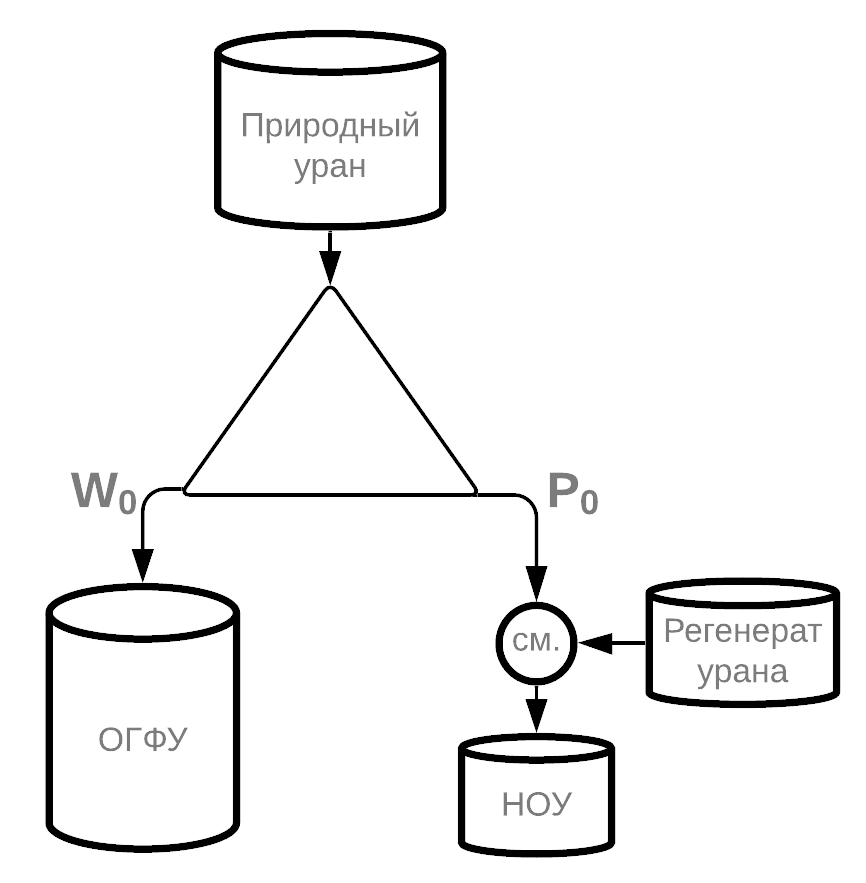
\includegraphics[scale=0.2]{cascades/ordinary/2}}
  \caption{Схема каскада с разбавлением предварительно обогащенного природного урана регенератом. Обозначения: $P_0$ -- поток отбора легкой фракции каскада; $W_0$ -- поток отвального ОГФУ тяжелого <<конца>> каскада; $CM.$ -- узел смешения, на выходе из которого получается конечный НОУ-продукт $НОУ$  -- низкообогащенный уран}\label{o2}
\end{figure}

Из результатов вычислительных экспериментов следует, что для рассматриваемой схемы с разбавлением предварительно обогащенного природного урана регенератом, принимая жесткие требования к четным изотопам, возможно получение решения, удовлетворяющего заданным условиям. Однако, как и в случае применения схемы рис. \ref{o1}, не удается добиться условия возврата заданной пропорции регенерата, так как в найденном решении недостаточен расход регенерата на единицу НОУ-продукта и составляет ($\approx$0,75). При этом уровень обогащения природного урана в каскаде достигает $\approx$16\% при различных значениях концентрации $^{235}$U в отвале этого каскада. Следовательно, как показано на примере изотопного состава регенерированного урана второго рецикла, такая схема обогащения регенерата не решает поставленную задачу для произвольного изотопного состава регенерата.

\subsection{Анализ схемы с разбавлением регенерата природным ураном перед подачей в ординарный трехпоточный каскад}

Еще одним вариантом реализации простейшей модификации ординарного каскада, используемого для обогащения природного урана, является предварительное смешение природного урана с регенератом перед подачей в каскад. Такая схема изображена на рис. \ref{o3}. Пропорция смешения сырьевых природного и регенерированного урана  определяется предварительно исходя из ограничений на четные изотопы в конечном НОУ-продукте.

\begin{figure}[ht]
  \centerfloat{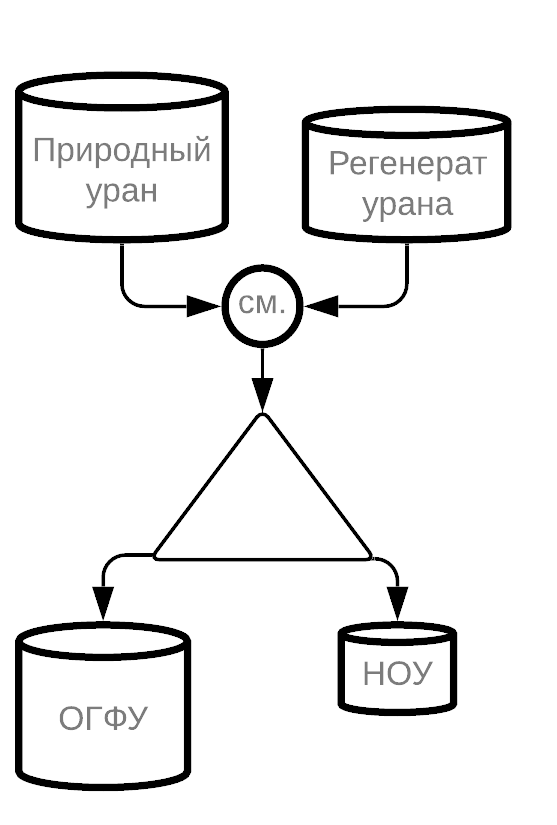
\includegraphics[scale=0.25]{cascades/ordinary/3}}
  \caption{Схема каскада со смешением регенерата и природного урана перед подачей на питание ординарного каскада. Обозначения: $P_0$ -- поток отбора легкой фракции каскада; $W_0$ -- поток отвального ОГФУ тяжелого <<конца>> каскада; $CM.$ -- узел смешения входящих сырьевых потоков; $НОУ$ -- конечный НОУ-продукт схемы}\label{o3}
\end{figure}

Как показывает анализ поиска решений схемы с разбавлением регенерата природным ураном перед подачей на питание каскада (рис. \ref{o3}), при использовании состава регенерата второго рецикла, в этом каскаде также невозможно достижение требуемой пропорции расхода регенерата урана на единицу финального продукта (рис. \ref{sc3_1.second}). Для каждого рассматриваемого значения концентрации $^{235}$U в $W_0$, имеется единственно возможное решение системы двух нелинейных уравнений, где обе невязки $\delta_1$ и $\delta_2$  обращаются в нуль, и в этих решениях, расход регенерата на единицу продукта ($\frac{RepU}{LEU Produce}$) не превышает 80\% от исходного. Эти решения изображены на пересечения кривых (рис. \ref{sc3_1.second}) с вертикальными и горизонтальными прямыми для указания на принимаемые ими значения расхода регенерата на единицу продукта ($\frac{RepU}{LEU Produce}$), а также доли регенерированного урана в смеси, питающей каскад ("RepU fraction in feed" на верхней горизонтальной оси).


\begin{figure}[ht]
  \centerfloat{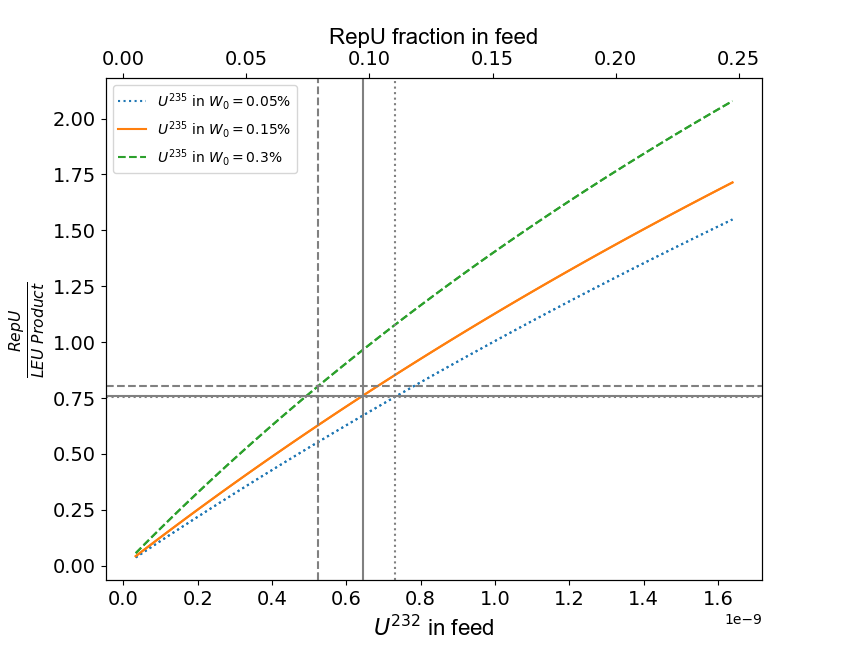
\includegraphics[scale=0.5]{images/plots/sc3_1.second}}
  \caption{Расход регенерированного урана на единицу НОУ-продукта  при различной концентрации $^{232}$U в питающем потоке каскада для различных концентраций $^{235}$U в потоке отвала}\label{sc3_1.second}
\end{figure}

% Рис.\ref{sc3_2.second} показывает расход природного урана на единицу продукта для того же набора найденных решений.

% \begin{figure}[ht]
%   \centerfloat{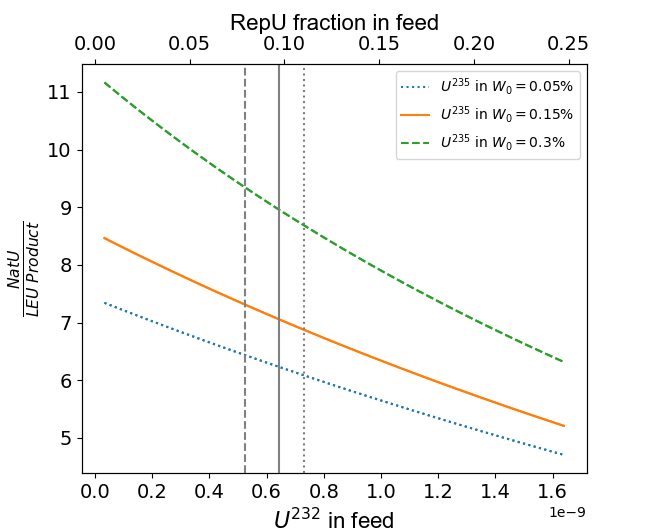
\includegraphics[scale=0.5]{images/plots/sc3_2.second}}
%   \caption{Расход природного урана на единицу НОУ-продукта  при различной концентрации $^{232}$U в питающем потоке каскада для различных концентраций $^{235}$U в потоке отвала}\label{sc3_2.second}
% \end{figure}


\subsection{Общий вывод для схем возврата регенерата в ЯТЦ на основе ординарного каскада}

Проведенные для схем на основе простейших модификаций ординарного каскада численные эксперименты показали, что такие схемы нецелесообразно использовать для вовлечения всего регенерированного урана в ЯТЦ в условиях многократного рецикла. Это происходит из-за ухудшения изотопного состава урана по мере прохождения им серии топливных циклов, что выражается в накоплении $^{232}$U. При этом исходная концентрация $^{232}$U питающей смеси, начиная со второго рецикла, превышает уровень допустимый в конечном продукте, поэтому схемы, основанные на ординарном каскаде, которые только разбавляют этот изотоп, не эффективны для решения поставленной задачи.

При этом закономерно возникает следующий вопрос: возможно ли априорно оценить способность рассматриваемой схемы решить поставленную задачу? 

Как следует из уравнений балансов материальных потоков \ref{GrindEQ__1_21_} путем предельного перехода получим частный случай балансового уравнения для самого легкого изотопа $^{232}$U \ref{eq_232_balance}. Из этого уравнения следует, что задействование массы регенерата близкой к массе получаемого продукта ($\approx$0,9-0,95) может быть обеспечено только тогда, когда концентрация $^{232}$U в исходном регенерате ниже, чем ограничение на $^{232}$U в конечном НОУ-продукте. 


\begin{equation}
\label{eq_232_balance}
  C_{232_{U}}^{P} \approx \frac{F}{P} C_{232_{U}}^{F}
\end{equation}

С помощью уравнения \ref{eq_232_balance} можно вычислить максимально возможную долю питающего потока, содержащего $^{232}$U, как неизвестную переменную уравнения \ref{eq_232_balance}. При этом предполагая, что весь исходный $^{232}$U окажется в конечном счете в продукте, так как его относительный коэффициент обогащения является самым высоким для смеси изотопов регенерата в виду того, что $^{232}$U является самым легким изотопом. На основе состава регенерата второго рецикла получаем \ref{eq_232_balance_X}:

% \begin{equation}
%   \label{eq_232_balance_X}
%     5 \times 10^{-7} \% \approx X \times 6.622 \times 10^{-7} \% \Rightarrow X \approx 0.755
% \end{equation}

\begin{equation}
  \label{eq_232_balance_X}
    \frac{RepU}{P} \approx 0.755
\end{equation}

Но, так как $\frac{F}{P}$ требуется на уровне $\approx$0,9-0,95 для достижения условия, накладываемого учетом за оборотом ядерных материалов, можно сделать вывод, что полностью вернуть регенерат в топливный цикл с помощью схем на основе простейших модификаций ординарного каскада в условиях многократного рецикла невозможно, так как начиная со второго рецикла, концентрация $^{232}$U в регенерата превышает пороговое значение для НОУ $5\cdot10^{-7}$\%.

В качестве следующей аналитической оценки, вычислим предельный вклад $^{235}$U в НОУ-продукт от используемого регенерата. На этот раз необходимо учитывать концентрацию $^{235}$U и в потоке отвала (ОГФУ), так как некоторое количество этого изотопа попадает в отвал каскада. Из балансных уравнений \ref{GrindEQ__1_21_} на основе данных концентрации $^{235}$U в составе регенерата второго рецикла, а также полученной выше достижимой пропорции  $\frac{F}{P} = \approx 0.755$, получаем:

\begin{equation}
  \label{eq_235_balance_X}
    \frac{\frac{RepU}{P}C_{4}^{RepU}}{\frac{X}{P}C_{4}^{P}} \Rightarrow X \approx 0.28\;,\; где\;i=4\;соответствует\;^{235}U
\end{equation}

% \begin{equation}
%   \label{eq_235_balance_X}
%    \frac{P*C_{235}^{P} - F_{регенерат}*C_{235}^{F_{регенерат}}}{P*C_{235}^{P}} \approx 0.0078
% \end{equation}

% Отсюда, сравнивая полученное значение с требуемой концентрацией $^{235}$U, можно вычислить предельный вклад $^{235}$U от регенерата, который будет составлять $\approx$16\% ($0.0078/0.0495\approx0.16$), что соответствует экономии природного урана. В реальной задаче, к сожалению, эта величина экономии будет еще меньше из-за необходимости компенсации по $^{236}$U.

величину предельного вклад $^{235}$U в НОУ-продукт от регенерата, который будет составлять $\approx$28\% . В реальной задаче, к сожалению, эта величина будет меньше из-за необходимости компенсации $^{236}$U.

Полученные аналитические оценки позволяют оценить возможность применения схем на основе простейших модификаций ординарного каскада, исходя из изотопного состава регенерата.Для рассматриваемого случая такие оценки позволяют априорно заключить, что, поскольку количество $^{232}$U в исходном регенерате второго цикла превышает ограничение в $5\cdot10^{-7}$\%, невозможно обеспечить возврат регенерированного урана в ЯТЦ в условиях многократного рецикла с помощью простейших модификаций ординарного каскада.


Таким образом, использование схем, ограниченных возможностью осуществлять разбавление четных изотопов исходной смеси регенерата, не позволяют решить задачу возврата регенерата в условиях многократного рецикла. Отсюда возникает потребность в модификации разделительного оборудования в контексте многократного рецикла урана, что и составляет цель диссертационной работы.


\section{Обоснование необходимости составных схем}\label{sec:ch2/sec2}

Как следует из вышеприведенных расчетов, на текущий момент имеются способы, позволяющие принципиально решить проблему выполнения требования по четным изотопам урана при обогащении регенерата, и основной проблемой, решаемой в рамках настоящей диссертационной работы, является поиск варианта каскадной схемы, позволяющей одновременно выполнить условия по четным изотопам и задействовать в обогащении весь имеющийся регенерат. В условиях разброса диапазона изменения состава.???

Если анализировать причины невозможности возврата регенерата в производство топлива в многочисленных модификациях каскада для обогащения многократно облученного регенерата, то становится очевидным, что это, во многом, связано с нарастанием относительных концентраций “легких” изотопов (в первую очередь $^{232}$U) и
$^{235}$U, а поскольку данные изотопы концентрируются вместе на легком <<конце>> каскада, то единственным способом понизить отношение их концентраций -- это разбавить материалом, не содержащим $^{232}$U, например на входе в каскад. Как показали результаты, описанных в этой главе вычислительных экспериментов, для составов с достаточно высоким исходным содержанием $^{232}$U невозможно подобрать такой разбавитель, чтобы удовлетворить одновременно и условие полного возврата регенерата в цикл и условия на содержание четных изотопов.

Из приведенного выше анализа вытекает необходимость использовать каскады, предназначенные для отделения друг от друга изотопов легкой фракции: $^{232,233,234}$U и более тяжелой: $^{235,236,238}$U. Такие схемы могут быть основаны на двух связанных каскадах, где в первом каскаде изотоп $^{235}$U обогащается с одновременным увеличением концентрации изотопов $^{232}$U и $^{234}$U, а во втором каскаде смесь изотопов разделяется на легкую ($^{232,233,234}$U) и тяжелую фракции ($^{235,238}$U) (рис. \ref{fig:double_ru}) \cite{smirnovApplyingEnrichmentCapacities2018}.

% Дальнейшая работа предполагает с использованием вычислительного эксперимента проведение анализа закономерностей массопереноса в каскадах, которые могут быть использованы для обогащения регенерированного урана в рамках многократного рецикла, для выработки рекомендаций к их применению.


% Из вышеприведенного обоснования невозможности решения задачи полного возврата регенерата в топливный цикл легководных реакторов в условиях многократного рецикла и вытекает необходимость использовать составные каскадные схемы ввиду необходимости  <<пространственного>> разделения легкой изотопной фракции с $^{232}$U, $^{234}$U от с $^{235}$U. Так двойная схема позволяет отделить минорные легкие изотопы $^{232}$U, $^{234}$U в независимом потоке отборной части каскада.
% Так, например, схема (рис. \ref{fig:double_ru}) позволяет во втором каскаде разделить потоки, выделив $^{235}$U в тяжелой фракции, направив $^{232}$U и $^{234}$U в легкую.
% С появлением свойств такого рода у каскадов, вместо привычной дихотомии, выделяющей схемы с приставкой <<много->> (многопоточные схемы, многокаскадные конфигурации), предлагается классифицировать каскады, используемые для обогащения регенерата, как разбавляющие или очищающие, потому что условная граница <<каскад-разбавитель>> -- <<каскад-очиститель>> гораздо лучше подчеркивает сущностные характеристики анализируемых схем, предназначенных для повторного обогащения урана. Так, схема двойного каскада является очищающей, в отличие от схем, основанных на ординарном каскаде, работающих на принципе разбавления.  

% В обзоре (глава 1) диссертации было показано, что такая схема (рис. \ref{fig:double_ru}) не может обеспечить соблюдение заданной пропорции для возврата.

\clearpage
